\chapter{ALGORITMA IZVĒRTĒJUMS} \label{algorithm-eval}


\section{Datu apstrādes tehniskā informācija}


Ņemot vērā, ka VSRC pārvaldībā ir nonācis jauns skaitļošanas klasteris, bija iespēja pielietot algoritmu uz jaunas paaudzes skaitļošanas klastera. Līdz ar to, bija iespējams veikt veiktspējas testus uz lielāka resursu daudzuma, salīdzinot ar parasti pieejamo, un apskatīt algoritma veiktspēju atkarībā no dažādu parametru konfigurācijas. Lai vairāk kontrolētu datu apstrādes vidi, tika izmantotas virtuālās mašīnas uz VSRC skaitļošanas klastera.


\begin{table}[h!]
\centering
\caption{Veiktspējas testos izmantoto individuālo virtuālo mašīnu apraksts}
\begin{tabular}{|l|l|}
        \hline
        Procesora ligzdas & 2 \\ \hline
        Procesora kodoli ligzdā & 48 \\ \hline
        BIOS   & SeaBIOS    \\ \hline
        Procesora tips    & kvm64   \\ \hline
        Atmiņa & 325.96 GB                    \\ \hline
        \end{tabular}
        
        \label{tab:vm-info}
\end{table}


Balstoties uz to, ka klastera mezgli izmanto \textit{Proxmox} operētājsistēmu, kas piedāvā iebūvētas virtuālo mašīnu veidošanas tehnoloģijas, tika izveidotas trīs virtuālās mašīnas ar tabulā \ref{tab:vm-info} aprakstītajiem parametriem. Virtuālajām mašīnām tika ielādēta \textit{Ubuntu 19.10 Live Server} versija, kā arī papildus noklusējuma bibliotēkām, tika instalētas \textit{openmpi} pakotnes, kā arī nepieciešamās bibliotēkas datu apstrādes skripta realizācijai. Skaitļošanas mezgli savā starpā saslēgti izmantojot 10GB/s optiskos kabeļus. Dati atrodas ārējā datu serverī, kas pieslēgts katrai virtuālajai mašīnai. Lai veiktu veiktspējas testus, tiek izmantoti dati no 2.2. nodaļā aprakstītā novērojuma.


\section{Veiktspējas testi}

Veicot veiktspējas testus, ir jāņem vērā daudz faktori, līdz ar to ideālu veiktspējas testu izpilde nav viegla. Faktori, kā ielasīšanas ātrums ir noteicoši konkrētā veida datu apstrādes algoritmos, līdz ar to ir limitācijas, cik ļoti ir iespējams uzlabot algoritma veiktspēju. Izveidojot pilnībā simulētu vidi, zūd algoritma veiktspējas uzticamība, salīdzinot ar veiktspēju reālajā pasaulē.

Veiktspējas testi ir veikti, izmantojot \textit{Linux} pakotni \textit{hyperfine}\cite{hyperfine}. Pakotne veidota, lai ērti nodrošinātu veiktspējas testu veikšanu, izmantojot nepieciešamos parametrus. Lai iegūtu salīdzinoši kontrolētus rezultātus, visiem nodaļā aprakstītajiem veiktspējas testiem tiek izmantotas 5 \textit{warmup} iterācijas, kā arī 30 rezultātu mērītās iterācijas.

Lai vieglāk atsauktos uz algoritma versijām, kuras tiek apskatītas, nodaļas ietvaros \textit{pirmā} versija MPI algoritmam apzīmē 1.5 nodaļā aprakstīto pirmo algoritmu, kurš attēlots pielikumā \ref{appendix:old-version}, bet \textit{pēdējā} versija apzīmē 1.5 nodaļā aprakstīto otro algoritmu, kurš attēlots pielikumā \ref{appendix:new-version}.

Lai attēlotu veiktspējas uzlabojumus no \textit{pirmās} MPI algoritma algoritma iterācijas un \textit{pēdējās}, ņemot vērā vienādu kodolu skaitu (9), rezultāti tiek atspoguļoti kastveida diagrammā \ref{fig:old-v-new} attēlā, kur ar violeto krāsu tiek attēloti rezultāti no \textit{pirmās} algoritma iterācijas, bet ar zaļo tiek attēlots \textit{pēdējās} algoritma iterācijas veiktspēja. Tehniski jēldatus \textit{pēdējā} versijā apstrādā par vienu procesu mazāk nekā \textit{pirmajā} versijā, taču tiek ņemts vērā, ka abi algoritmi katrs aizņem deviņus procesus kopā. 



Ņemot vērā, ka datos ir izlecošās vērtības, biežākais izpildes laiks tiek mērīts, izmantojot mediānas vērtību. Pēc veiktspējas testu rezultātiem, \textit{pirmās} versijas algoritms visbiežāk izpildīsies aptuveni 3193.2148 sekundēs, kamēr \textit{pēdējā} algoritma versija izpildīsies aptuveni 2535.8932 sekundēs. 


Jāņem arī vērā, ka \textit{pirmajā} algoritmā nav integrētas anomāliju pārbaudes, kuras aprakstītas nodaļā \ref{anomalies}, kā arī papildus datu izveide, līdz ar to, ja \textit{pēdējā} algoritma darba skaits tiktu pielīdzināts \textit{pirmajam}, tā veiktspēja būtu vēl sliktāka. Lai gan \textit{pirmā} algoritma darbībai, pēc teorijas, vajadzētu būt ātrākai, \textit{pēdējā} algoritma ietvaros tiek izmantoti dažādi augstas veiktspējas risinājumi problēmām, it īpaši ciklu vektorizācija, kas izteikti minimizē darbību ilgumu.

\begin{figure}[H]
\centering
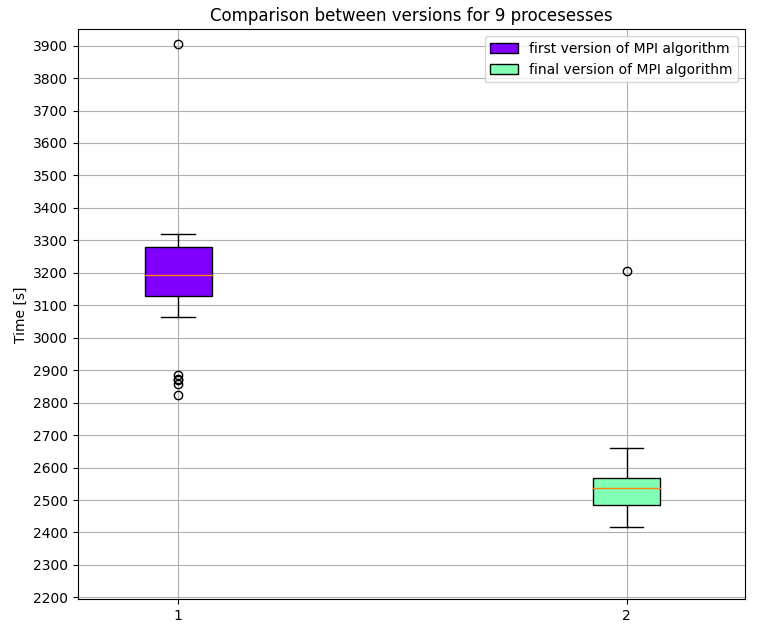
\includegraphics[width=\textwidth]{images/created/old-v-new.png}
\caption{Pirmā datu apstrādes algoritma veiktspējas salīdzinājums ar pēdējās versijas veiktspējas salīdzinājumu.}
\label{fig:old-v-new}
\end{figure}


\textit{Pēdējais} algoritms ir tieši atkarīgs no procesu skaita un failu daudzuma. Ideālā gadījumā, datu apstrādē algoritmam būtu iespējams  apstrādāt katru failu savā procesā, taču, lai to realizētu 4 stundu gariem novērojumiem, būtu nepieciešams paredzēt 1920 kodolus datu apstrādei, kas patreizējā situācijā ir reti iespējams. Pēc teorijas, palielinot kodolu daudzumu, izpildes laiks samazināsies.

Lai attēlotu \textit{pēdējās} versijas algoritmu, tiek apskatīts veiktspējas rezultāts atkarībā no pieejamiem resursiem. Attēlā \ref{fig:all-bench} tiek atspoguļoti rezultāti izmantojot 9, 64, 192 un 234 procesus. Iegūtie rezultāti no 9 un 64 procesu datiem ir apstrādāti vienas virtuālās mašīnas ietvarā, bet 192 un 234 procesu rezultāti, izmantojot visu virtuālo mašīnu kopējos skaitļošanas resursus. 






\begin{figure}[H]
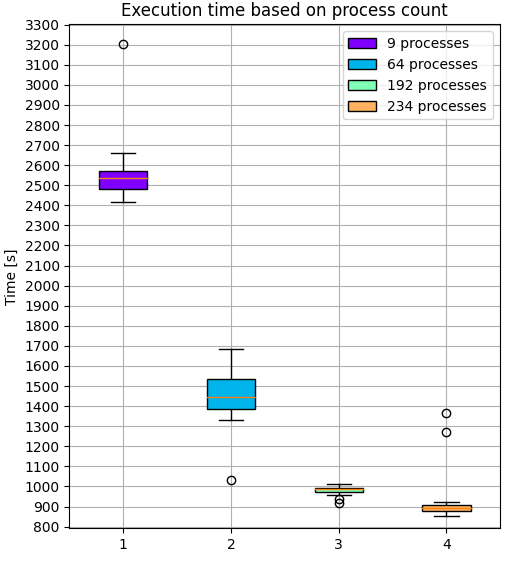
\includegraphics[width=\textwidth]{images/created/all-bench-rez.png}

\caption{\textit{Pēdējā} algoritma veiktspēja atkarībā no procesu skaita}
\centering
\label{fig:all-bench}
\end{figure}

Lai gan Bakalaura darba ietvaros nav apskatīts pats sākotnējais algoritms, kurš realizēts bez MPI iekļaušanas, tipiska novērojuma apstrādāšanai bija nepieciešamas aptuveni 5 stundas.



\section{Algoritma potenciālie uzlabojumi}

Algoritma veiktspējas uzlabošanas lielākais šķērslis ir algoritma procesu pārvaldības procesa optimizācija, jo apskatot kodolu noslodzi, var noteikt, ka algoritma izpildes sākuma posmā visi izsauktie kodoli izpildās uz 100\% noslodzi, taču, kad pirmie faili nolasīti, uz pārvaldības procesu vienlaicīgi tiek sūtītas vairākas ziņas no apstrādes procesiem par nolases pabeigšanu. Tas nozīmē, ka ir nepieciešams apstrādāt visus ienākošos procesus, piešķirot atbrīvojušajiem procesiem jaunu failu apstrādei, kā arī klausīties jeb nodrošināt pārējo procesu statusu monitoringu. Visas aprakstītās darbības prasa skaitļošanas laiku, līdz ar to nevar efektīvi pārvaldīt visus pieejamos procesus. Problēmas risinājums būtu ieviest vairāk-pārvaldības procesus, lai gan minētais uzlabojums varētu ļoti sarežģīt algoritma loģiku. Lai gan patreizējā \textit{numpy} vektorizācija ir daudz efektīvāka, salīdzinot ar ciklu pieeju, ir ieteicams izmantot iebūvētās \textit{MPI} funkcijas, kuras nodrošinātu efektīvāku procesu komunikāciju.



Veicot datu apstrādes algoritmu optimizāciju, ir iespējams izmantot divas pieejas, kur katrai ir savi izmantošanas plusi un mīnusi. Pirmā pieeja, kuru savā ziņā arī izmanto \textit{pirmais} MPI algoritms, ir statiski norādīt instrukcijas katram procesam un katru reizi algoritma izpildē izmantot statisku procesu daudzumu. Minētais risinājums ļoti uzlabo kopējo veiktspēju, jo tiek samazināts komunikāciju daudzums starp procesiem, kā arī realizācija ir daudz vienkāršāka, izmantojot nemainīgas instrukcijas, tādējādi veidot pilnībā kontrolētu vidi. Bet kopumā aprakstītais risinājums padara algoritmu nemērogojamu. Izmantojot \textit{pirmo MPI} algoritmu, nav iegūti augstākas veiktspējas rezultāti par jaunākās versijas rezultātiem, jo starp iterācijām tika apgūtas dažādas augstas veiktspējas labās prakses, kas krasi uzlaboja veiktspēju.

Ņemot vērā, ka pieejamais skaitļošanas resursu daudzums var mainīties, nav garantēts konkrēts kodolu skaits algoritma izpildei, bija nepieciešams izmantot otro pieeju - zaudēt statiskās instrukcijas katram procesam un dinamiski atļaut procesu pārvaldību. Minētā pieeja vienmēr samazinās kopējo veiktspēju, jo procesiem savā starpā jāsazinās un jāinformē par procesa stāvokli, bet visbiežāk, izveidojot algoritmu pēc minētās metodes, ir iespējams iegūt labāku veiktspēju kopumā, vienkārša iemesla dēļ - programrisinājumam ir pieejami vairāk skaitļošanas resursi.

Ņemot vērā, ka Bakalaura darba ietvaros koda optimizācija un kopējā veiktspēja ir svarīgs faktors, jāņem vērā, ka patreizējā sistēma pilnībā ir realizēta Python programmēšanas valodā. Tā tika izvēlēta atvieglotai algoritma realizācijai, plašo bibliotēku atbalsta un vienkāršotās sintakses dēļ, bet valodai dēļ tās izpildes laika interpretatora ir izteiktākas tehniskās limitācijas. Izmantojot \textit{numpy} bibliotēku var efektīvi vektorizēt darbības, kā ciklu izpildi un matricu manipulāciju, bet pilnībā optimizēts kods visticamāk būs lēnāks par pilnībā optimizētu kodu zemāka līmeņa valodā, kā C, pateicoties faktam, ka kods tiek interpretēts izpildes laikā. Diemžēl nav iespējams izvērtēt algoritma pārrakstīšanas guvumu neieguldot daudzas stundas pārrakstīšanā, līdz ar to konkrētus rezultātus konkrētajā jautājumā nevar iegūt.
